\section{Material and Methods}
\label{MaterialandMethodsMedianMedia}

\subsection{Data collection and sampling design}

Data collection included 540 observations distributed evenly among 10 locations on two islands. Two cities on two different islands within the Central-Southeastern zone of the Galapagos archipelago, which were expected to have significantly different levels of anthropogenic pollution, were selected; Puerto Ayora (Academy Bay) on Santa Cruz island and Puerto Velazco Ibarra on Floreana island. Puerto Velazco Ibarra is the smallest city of the archipelago with 111 inhabitants, while Puerto Ayora is the largest city with 11822 inhabitants and the highest number of visiting tourists, according to a survey of 2015 \citep{INEC2015Censo2015}. Per city, five locations with rocky habitats were chosen along the coast to use fixed video transects to study fish assemblages. Video transects were chosen over traditional visual census techniques, as the former allows to (i) store video data for later analysis, (ii) reduce the amount of time spent on field work and (iii) improve the standardization of data collection \citep{Mallet2014,Wartenberg2015}. The fish data collection was based on a standard operation procedure developed by the Aquatic Ecology Research Group of Ghent University (see further). On each location, three transects with a length of 50 meters each were laid out using ropes. For fish to be included they had be recorded within 2.5 m of either side of the transect line (area = 50 x 5 = 250 m$^{2}$). Observers were trained to recognize whether fish had to be considered, depending on the estimated distance from the rope. All transects were monitored at a constant depth of 1.5 meters, parallel to the coastline, and only locations with a limited exposure to waves were selected to guarantee the safety of the observers and to avoid predominant effects of wave exposure on the structure of fish assemblages. All transects were approximately 20 meters apart. In practice, this meant that transects were placed next to each other along the coastline. To account for observer bias and sampling variability, each of these transects was recorded six consecutive times with single GoPro cameras (GoPro Hero 5 Black, 1080p, 60fps, wide FOV) by three different observers equipped with a mask and snorkel. Hence, ten locations x three transects x three observers x six repeats yielded 540 observations (18 per transect) (Figure S1.1). In summary, two islands, with five locations each, were studied. In each location, three transects were each covered six times by each of the three observers.

The observers covered the transects in a browsing fashion, similar to the S-type transects introduced by Pelletier et al. (2011) \citep{Pelletier2011}. Observers browse through the transect at a fixed speed, but varying angle and can zoom in if needed to find individuals hiding in crevices. This S-transect was chosen over the more standarized I-transect with fixed angle and without zooming because the former had been found to enable detection of more individuals and species compared to the latter \citep{Pelletier2011}. Transects were placed during low tide and monitored during flood tide of consecutive days from the $19^{th}$ until the $31^{st}$ of August 2017. The duration of each observation was approximately 4.6 minutes ($\pm 0.7$ minutes). The time between each observation was at least one minute and subsequent observations were found independent in terms of diversity and assemblage structure (section S2). Per day one location was monitored. The analysis of the videos included species identification and an estimation of the number of individuals per species, determined as MaxCount, i.e. the total number of individuals per species per observation. The videos were analyzed once by one out of two video analysts; videos were assigned randomly to these analysts to reduce inter-observer bias \citep{Williams2006ImpactSurveys}. 

Halfway the biological monitoring of a specific location, physical-chemical conditions were determined once using in situ measurements. In situ measurements were based on standard operation procedures developed in the Aquatic Ecology Research Group of Ghent University. Water temperature, acidity (pH), electrical conductivity (EC), dissolved oxygen (DO) and chlorophyll were measured with handheld multiprobes (WTW for temperature ($^{\circ}$C), pH (-) and DO concentration (mg L$^{-1}$); Aquaread (AP5000 version 4.07) for EC (mS cm$^{-1}$) and chlorophyll (\SI{}{\micro\gram} L$^{-1}$)). Due to unstable measurements, chlorophyll concentrations were only used to compare average values of both islands and were not considered as a parameter in the constructed models. Nutrient concentrations of nitrite (mg NO$_{2}^{-}$-N L$^{-1}$), nitrate (mg NO$_{3}^{-}$-N L$^{-1}$), ammonium (mg NH$_{4}^{+}$-N L$^{-1}$), sulfate (mg SO$_{4}^{2-}$ L$^{-1}$), phosphate (mg PO$_{4}^{3-}$-P L$^{-1}$), total phosphorus (total P) (mg P L$^{-1}$) and total nitrogen (total N) (mg N L$^{-1}$) were determined spectrophotometrically (ThermoFisher Genesys 10S UV‐VIS) using Merck kits. Measurements that were below the detection limit, were given the value of the detection limit. This was only the case for ammonium concentrations in Floreana and at location B10 in Santa Cruz, which were given a value of 0.01 mg NH$_{4}^{+}$-N L$^{-1}$. To assess how the anthropogenic influences differed between islands, in five locations in Floreana and three locations in Santa Cruz, the presence/absence of coliforms and \textit{Escherichia coli} was determined as a measure of fecal contamination. To assess the underlying causes of patterns in water quality (i.e. variability in natural conditions or variability in anthropogenic pollution) satellite imagery and simulations from remote sensing based models were used. Results suggested that Floreana has lower levels of anthropogenic pollution but more clear signs of natural upwelling than Santa Cruz. More information is provided in section S3. 

For each transect the percentage cover of different habitat classes (i.e. bare rock, rock with sediment deposition, vegetated rock and sand) was determined within 2.5 meters of each side of the rope through visual inspection of the video data. Physical habitats are often complex and difficult to classify. Therefore, each transect was covered multiple times to assess how closely fish assemblages were associated with a specific (series of) micro-habitat(s). Since the scale and the intensity of the biological and environmental sampling differed, the biological data was aggregated to the level of transects (30 transects, i.e. 2 islands x 5 locations x 3 transects) to fit the scale of the abiotic data before applying constrained ordination. In addition, because of the spatially nested nature of the data, the geographical distances between sampling units (i.e. transects) were at significantly different scales (i.e. between islands, between locations and between transects). Therefore, similarities between nearby locations and transects may be the result of the spatial structuring of species distributions rather than local environmental conditions \citep{Guisan2006,Kissling2008SpatialModels,Legendre1993SpatialParadigm}. This spatial structuring, which manifests itself in the data as spatial auto-correlation, was accounted for by explicitly integrating the geographical distance between the sampling units in the different models \citep{Legendre1993SpatialParadigm}. 

To aggregate the biological data within transects the median of the 18 observations per transect was chosen over the mean or maximum. Since fish tend to be very mobile, occasional observations of different species moving between locations, may yield questionable results. Using the median rather than the mean accounts for this bias, though it comes at a cost, since individuals of cryptic, rare and easily scared species will also be less likely to be observed during multiple observations.

\subsection{Data analysis}

All analyses were performed using the R software \citep{RCoreTeam2019R:Computing} and the Primer v6 multivariate statistics package \citep{Clarke2006PRIMERManual/Tutorial} with PERMANOVA add-on \citep{Anderson2008PERMANOVA+Methods}. In Figure S1.2, the data analysis roadmap is presented. 

\subsubsection{Spatial variability of water conditions and habitats}
\label{Methods:env_grouping}

In this study, geographical distance, i.e. normalized longitude (X) and latitude (Y), was used to account for spatial auto-correlation and dispersal. The distances between the locations within one island were negligible compared to the distance between the two islands. Despite the aim of selecting locations at similar distances of each other, due to logistic constraints this was not always possible. In Floreana, the locations were more or less at equal distances from each other along the coast, but this was not the case for Santa Cruz, where locations were positioned within a bay, spatially clustering locations B2 and B3 as well as B9 and B10, while B6 was more isolated (Figure \ref{fig:MAP}). The average distance between locations for Santa Cruz and Floreana was 734 $\pm$ 544 meters (SD) and 525 $\pm$ 397 meters (SD), respectively. 

DISTLM (see further) does not make any assumptions about the distributions of the covariables, but these distributions should nevertheless be appropriate for linear modelling \citep{Anderson2008PERMANOVA+Methods,Legendre1999Distance-basedExperiments}. Therefore, to assess whether distributions of covariables were not skewed or contained outliers, draftsman plots were constructed and analyzed. To deal with the detected skewness and outliers of some of the covariables, these were transformed before normalization (subtraction of mean and division by standard deviation). Nitrite, nitrate, ammonium, total N, total P, phosphate and DO concentration were log(V) transformed and sulfate concentration was -log(2-V) transformed. Similarly, the cover of different habitat classes was often left or right skewed. Therefore, the percentage cover of the physical habitats was arcsine square root transformed prior to conducting the analyses \citep{Gotelli2004AStatistics.}. The resulting histograms and residual plots indicated a better fit compared to the case of no transformation (tested for all covariables) or logit transformation (tested for the cover of the habitat classes).

Principal Component Analysis (PCA) was used to visually assess any potential grouping of the water variables and the physical habitats. Tests of homogeneity of dispersions (PERMDISP) based on Euclidean resemblance matrices of the physical habitats and water conditions allowed to determine and compare the variability of both series of environmental variables in both islands. Additional PERmutational Multivariate dissimilarity-based ANOVA (PERMANOVA) analyses allowed to assess whether physical habitats and water conditions were significantly different between islands and locations (nested in islands). The PERMANOVA analyses were done using 10$^{5}$ unrestricted permutations of the raw data. To compare the physical habitats of the islands, locations were considered as a random factor. To compare the physical habitats of the locations, one analysis was performed for both islands together. If both PERMANOVA and PERMDISP tests were found to be significant, additional Canonical Analysis of Principal coordinates (CAP) tests were used to assess the distinctiveness of the considered groups.   

\begin{figure}[h!]
  \centering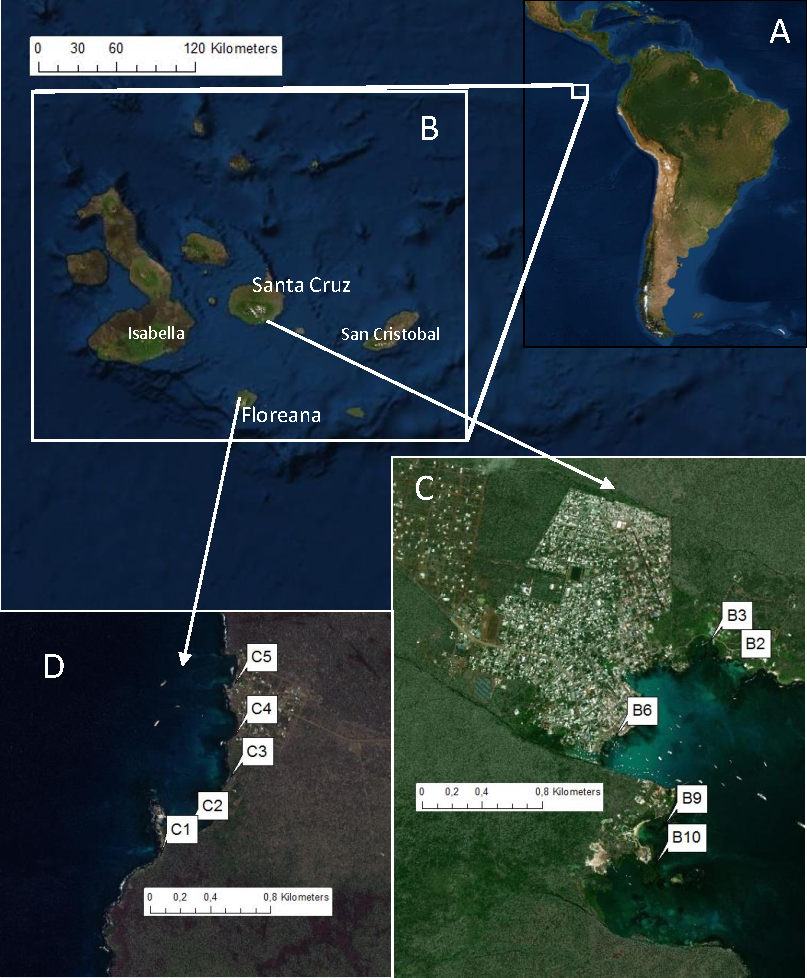
\includegraphics[scale=0.8]{MAP}
  \caption{Map of the study area. (A) South-American continent with depiction of the Galapagos archipelago. (B) Galapagos archipelago with depiction of the two studied islands. (C) The city Puerto Ayora on Santa Cruz island with indication of the study locations. (D) The city Puerto Velazco Ibarra on Floreana island with indication of the study locations. Landsat 8 imagery was used to construct the maps.} 
  \label{fig:MAP}
\end{figure}

\subsubsection{Fish $\alpha$ and $\beta$ diversity}
\label{sect:div}
 
In literature there have been many different definitions for both $\alpha$ diversity and $\beta$ diversity, underlining the importance of a clear description of the definition used in each study. In this study, we mainly adopted the definitions provided by Gray (2000) \citep{Gray2000TheShelf}, which are closely related to the original definitions provided by Whittaker (1975) \citep{Whittaker1975CommunitiesEcosystems}. The number of species observed per sampling unit is referred to as point species richness. Since it is unlikely that only one sampling unit would be representative for the entire study area, a sample typically comprises multiple sampling units within the area. The number of species found within a sample is referred to as sample species richness, which is more closely related to Whittaker's $\alpha$ diversity. In this study, the number of species observed during a single observation is defined as the point species richness, while the total number of species within an island, location or transect is referred to as the sample species richness. The sample species richness was assessed visually using Species Accumulation Curves (SACs) (10$^{5}$ permutations) for the different islands (n=270 per island) and locations (n=54 per location)\footnote{For each level of sampling effort, observations are resampled without replacement and the total number of different species over all considered observations per sampling event are counted. Finally, the average and confidence intervals of the 10$^{5}$ resampling events are determined for each level of sampling effort. The curvature provides insight in the expected species diversity \citep{Chao2004NonparametricSampling}}. SACs depict the number of observed species with increasing sampling effort and are typically used to estimate the number of species in a particular area \citep{Magurran}. To statistically compare the sample species richness of islands and locations (Wilcoxon rank sum tests) and to assess correlations with environmental variables, respectively the total number of observed species per location and transect (maximum sample species richness) were retained for analysis. To compare the point species richness of both islands, a linear mixed model with island as fixed effect, location and transects as nested random effects and observer as crossed random effect were constructed. To compare the point species richness of the locations, one analysis was performed for both islands together using a linear mixed model with location as fixed effect and transect and observer as nested and crossed random effects respectively. 

%$\beta$ diversity is broadly defined as the degree to which a set of samples in a given geographical area varies in the identities of the species they contain \citep{Whittaker1975CommunitiesEcosystems,Whittaker2001ScaleDiversity}. 
Although $\beta$ diversity can be defined in numerous ways, in this study it is defined as the variability in species composition among samples for a given area at a given spatial scale \citep{Anderson2006MultivariateDiversity,Whittaker1975CommunitiesEcosystems,Whittaker2001ScaleDiversity}. Differences in $\beta$ diversity at the spatial scale of (1) islands and (2) locations were assessed using a PERMDISP test on the Sorensen resemblance matrix of the samples, in which a sample corresponds with the aggregated data of a single transect. The distance to centroid in a two-dimensional Principal Coordinate (PCO) space is considered a measure of $\beta$ diversity \citep{Anderson2006MultivariateDiversity}. To compare (1) islands and (2) locations, the centroids of the samples of (1) each island and of (2) each location were used respectively. To assess if there were any relationships between environmental conditions and diversity, Pearson correlation coefficients (\textit{r}) of the diversity measures versus the transformed environmental variables were determined. 

\subsubsection{Fish assemblage structure}
\label{sect:struct}

Differences in the structure of fish assemblages between islands are not necessarily the result of their position along an environmental gradient, but rather the result of fragmentation due to migration barriers, local extinction or colonization \citep{Whittaker1998IslandConservation,Whittaker2017IslandLaboratories}. Therefore, parametric methods such as MANOVA, PCA, CCA and RDA, which assume an underlying environmental model of species distributions \citep{TerBraak1988AAnalysis}, are not appropriate. In addition, ecological data, especially those originating from visual census, are often overdispersed and zero-inflated, limiting the use of traditional parametric methods. On the other hand, purely non-parametric approaches, such as ANOSIM, are unable to partition variability, assess interactions or model more complex patterns \citep{Anderson2008PERMANOVA+Methods}. Semi-parametric multivariate techniques, such as PCO, PERMANOVA, CAP and dbRDA, combine the advantages of both approaches and rely on the actual values of the resemblance matrix instead of relative ranks, but still use permutations rather than distributional assumptions \citep{Anderson2008PERMANOVA+Methods}. Nevertheless, by using the actual dissimilarity values instead of ranks, the choice of transformation, aggregation and measure of resemblance become more important \citep{Anderson2008PERMANOVA+Methods}. 

The analyses were performed on the Bray-Curtis resemblance matrix of the original fourth-root transformed biological data set. Prior to applying PERMANOVA, a PERMDISP analysis was performed to test for homogeneity among the dispersions of the different islands and locations \citep{Anderson2015}\footnote{It should be noted that $\beta$ diversity was also assessed with a PERMDISP analysis, as it can statistically be represented as the multivariate dispersion of the Sorensen resemblance dissimilarity matrix (presence/absence) of the data (section \ref{sect:div}). However, in this section, dispersion was determined to assess whether PERMANOVA-violations took place. Hence, data transformation and the type of dissimilarity matrix used were the same as those used for the corresponding PERMANOVA (i.e. Bray-Curtis resemblance  matrix  of  the  original  fourth-root transformed data set). Throughout this work the term dispersion was used in the context of assessing any violations of model assumptions, while $\beta$ diversity was used to refer to a specific type of multivariate dispersion with predetermined settings.}. Although PERMANOVA is quite robust to heterogeneity of variances for balanced designs when compared to other methods such as ANOSIM or the Mantel test \citep{Anderson2016}, significant differences in multivariate variability may complicate interpretations of PERMANOVA analyses. More specifically, if both PERMDISP and PERMANOVA yield significant results, there is not necessarily a significant discrepancy in the structure of the fish assemblages other than the difference in variability. Therefore, additional CAP discriminant analyses were applied to assess the distinctiveness in the structure of fish assemblages between the islands, locations and transects. The leave-one-out misclassification error was used as a measure of the distinctiveness of each of the groups.

To compare islands using PERMANOVA, the considered factors were island (fixed), location (random and nested within island), transect (random and nested within location) and observer (random and crossed). To compare locations using PERMANOVA, irrespective of the islands, the factor island was dropped and the factor location was treated as the fixed factor. The assessment of the main effects and pair-wise comparisons were obtained using 10$^{4}$ permutations of residuals under a reduced model. The square root components of variation ($\sigma^{'}$) were estimated by equating the mean squares of the PERMANOVA models to their expectations \citep{Anderson2008PERMANOVA+Methods}. To determine the proportion of the variability explained by the different grouping factors, the percentage of variation of each component to the total variation was used. PCO analyses were performed to visualize the multivariate patterns. The fish species that were characteristic for the differences among the islands and locations were found by superimposing vectors corresponding to Pearson correlations of individual species with the resulting PCO axes.

CAP analyses were also performed to describe the correlation of the aggregated multivariate biological data to gradients of water variables, physical habitats and geographical distance. The first PCA axis, describing each series of variables, being habitat, water conditions and distance, was retained and plotted against the first CAP axis of the aggregated biological data set and the corresponding canonical correlation of both axes was determined.

To assess the relative importance and overlap of geographical distance, water conditions and physical habitats in shaping the observed fish assemblages, they were considered as separate subsets of variables in DISTance-based Linear Models (DISTLMs). While CAP finds linear combinations of the biotic and abiotic variables that are maximally correlated with one another, DISTLM finds linear combinations of the abiotic variables that are best to predict patterns in the biotic data set \citep{Anderson2008PERMANOVA+Methods}. As such, DISTLM models take into account the potential overlap of different predictors. Data was aggregated to the level of transects (median) and spatial auto-correlation was accounted for by explicitly integrating geographical distance. Because the number of spatial variables was limited compared to the number of variables of the other two series, the polynomials up to 3$^{rd}$ order of the coordinates, i.e. X (longitude) and Y (latitude), were included as well. Since the number of variables exceeded the amount of observations, no interactions were considered and subsets of variables were established for each series using forward selection based on the multivariate analogue to the small-sample-size corrected version of the Akaike Information Criterion (AICc) and sequential conditional distance-based Redundancy Analysis (dbRDA). To compare the series, ideally the number of variables per subset should be the same. However, the optimal number of variables based on the AICc can differ between the series. Therefore, the effect of including fewer or more variables was assessed and the variability of the results was evaluated (section S9). These subsets were then compared using the AICc values, forward selection and sequential conditional dbRDA. Models were also constructed for all variables independent of the series they were assigned to, using forward selection. Finally, this approach was extended by assessing all possible combinations of variables to construct q-variable models with q ranging from one to six.  

It is important to note that for the analyses that only considered biological data (i.e. PERMDISP, PERMANOVA, and CAP) the full biological data set was used (n=540), while for the analyses that considered both environmental and biological data (i.e. DISTLM and CAP-PCA) the aggregated biological data set was used (n=30).